\chapter{tirxBujAkAra saMkeyxgaLu}

oMdariMda AraMBavAguva karxmAgata saMKeyxgaLanunx kUDutAtx hoVdare baruva motatxkekx tirxBujAkAra saMkeyxgaLeMdu hesaru. I riVtiya saMKeyxgaLanunx tirxBujada rUpadalilx bareyabahudu AdadxriMdaleV I hesaru baMdide.

\begin{minipage}[c]{4cm}
\begin{flalign*}
&1=1&\\
&1+2=3\\
&1+2+3=6\\
&1+2+3+4=10\\
&1+2+3+\cdots n = \frac{n(n+1)}{2}\\
\end{flalign*}
\end{minipage}
\begin{minipage}[c]{5cm}
\text{ivugaLelalxvU {\bf tirxBujAkAra} saMKeyxgaLu}
\end{minipage}

ivugaLanunx $T(n)$ eMba cihenxyiMda sUcisutetxve.

\begin{minipage}[c]{5cm}
\begin{align*}
T(1) &= \frac{1\times 2}{2} =1\\
T(2) &= \frac{2\times 3}{2} =3\\
T(3) &= \frac{3\times 4}{2} =6\\
\end{align*}
\end{minipage}
\begin{minipage}[c]{5cm}
$\therefore T(n) = \frac{n(n+1)}{2}$
\end{minipage}

eraDu karxmAgata tirxBujAkAra saMKeyxgaLu vagaRsaMKeyxyanunxMTu mADutatx.
\begin{equation*}
\left.
\begin{aligned}
T(1)+T(2) &= 1+3 = 4\\
T(3)+T(4) &= 6+10 = 16
\end{aligned}
\qquad\right\}
\qquad\text{vagaRsaMKeyxgaLu}
\end{equation*}
\begin{align*}
T(n-1)+T(n) &= \frac{(n-1)n}{2} +\frac{n(n+1)}{2}\\
&= \frac{n^2-n+n^2+n}{n} = \frac{2n^2}{2}=n^2\\
\end{align*}

yAvudAdarU tirxBujAkArada saMkeyxya  $8$ raSaTxkekx $1$ nunx seVrisidare vagaRsaMKeyxyu pArxpatxvAgutatxde.
\begin{equation*}
\begin{aligned}
8T(1)+1 &=8+1 =9\\
8T(2)+1 &=24+1 =25\\
8T(4)+1 &=80+1 =81\\
\end{aligned}
\qquad\text{vagaRsaMKeyxgaLu}
\end{equation*}

\begin{align*}
8T(n)+1 &= \frac{8\cdot n(n+1)}{2}+1\\
&= 4n(n+1)+1\\
&=4n^2+4n+1\\
&=(2n+1)^2 \qquad \text{vagaR saMKeyx}
\end{align*}

$2\left\{100 T(n)+12\right\}+1$ eMba sUtarxvu vagaRsaMkeyxyanunx niVDutatxde.
\begin{equation*}
\begin{aligned}
n=1 \quad \text{AdAga} \quad &2\left\{100T(1)+12\right\}+1\\
       &=2\times 112+1 = 225\\[0.2cm]
n=1 \quad \text{AdAga} \quad &2\left\{100T(2)+12\right\}+1\\
       &=2\times 312+1 = 625\\[0.2cm]
n=1 \quad \text{AdAga} \quad &2\left\{100T(3)+12\right\}+1\\
 &=2\times 612+1 = 1225\\      
\end{aligned}
\qquad\text{ivelalxvU vagaRsaMKeyxgaLu}
\end{equation*}
I riVti laBayxvAda vagaRsaMKeyxgaLelalxvU $25$ ralilx konegANutatxve.
\begin{flalign*}
1^2&= 1&\\
3^2 &=1+8 =9\\
6^2 &= 1+8+27 =36\\
10^2 &= 1+8+27+64 =100
\end{flalign*}
aMdare karxmAgata tirxBujAkAra saMKeyxgaLa vagaRgaLu, karxmAgata Gana saMKeyxgaLa motatxkekx sama.

\begin{itemize}
\item[{\rm I}] tirxBujAkAra saMKeyxgaLanunx I riVti sUcisabahudu.
\begin{figure}[h]
\centering
\includegraphics{src/figure/m_071.eps}
\end{figure}
\item[{\rm II}] tirxBujAkArada saMKeyxgaLanunx I riVtiyalUlx sUcisabahudu.
\begin{figure}[h]
\centering
\includegraphics{src/figure/m_071a.eps}
\end{figure}
\end{itemize}

